\documentclass[modern]{aastex631}


\usepackage{amsmath}
\usepackage{amssymb}
\usepackage{hyperref}
\usepackage{bm}
\usepackage{listings}
\usepackage{graphicx}
\usepackage{float}
\usepackage{soul}
\usepackage{mathtools}
\usepackage{esint}

% missing figure command

\usepackage{blindtext}
\usepackage{graphicx}
\usepackage{tcolorbox}
\usepackage{fontawesome}
\usepackage{booktabs}

\definecolor{linkcolor}{rgb}{0.1216,0.4667,0.7059}


\let\StandardIncludeGraphics\includegraphics%
\renewcommand{\includegraphics}[2][]{%
\IfFileExists{#2}{%
  \StandardIncludeGraphics[#1]{#2}%
}{%
 \IfFileExists{#2.pdf}{%
  \StandardIncludeGraphics[#1]{#2}%
  }{ % No, no .pdf, try *.jpg 
   \IfFileExists{#2.jpg}{%
    \StandardIncludeGraphics[#1]{#2}%
    }{
      \IfFileExists{#2.png}{%
      \StandardIncludeGraphics[#1]{#2}%
      }{%
      \begin{tcolorbox}[width=6cm,height=4cm,arc=0mm,auto outer arc]
      \end{tcolorbox}
     }
   }
 }
}% 
%
}

% commands
\newcommand{\todo}[1]{\colorbox{red}{\textcolor{white}{\texttt{TO DO}}}\,}
\newcommand{\set}[1]{\{\,#1\,\}}
\newcommand{\footlink}[1]{\footnote{\url{#1}}}
\DeclareMathOperator*{\argmax}{arg\,max}
\DeclareMathOperator*{\argmin}{arg\,min}
\let\subsectionautorefname\sectionautorefname
\let\subsubsectionautorefname\sectionautorefname
\newcommand{\codeicon}{{\color{linkcolor}\faFileCodeO}}
\newcommand{\codelink}[1]{\href{https://github.com/lgrcia/paper-jaxoplanet/blob/main/#1.py}{\codeicon}\,\,}
\newcommand{\gitlink}{\href{https://github.com/lgrcia/paper-jaxoplanet}{\color{linkcolor}\faGithub}\,\,}

% no indent
\setlength\parindent{0pt}

% code style
\lstdefinestyle{mystyle}{
    backgroundcolor=\color{white},
    commentstyle=\color{gray!70},
    keywordstyle=\color{Bittersweet},
    stringstyle=\color{RoyalBlue},
    basicstyle=\fontsize{8.5}{13}\fontfamily{DejaVuSansMono-TLF}\selectfont,
    breakatwhitespace=false,         
    breaklines=true,
    rulecolor=\color{black!15},
    numbers=none,
    numberstyle=\fontsize{7}{11}\fontfamily{DejaVuSansMono-TLF}\selectfont\color{gray!50},
    framerule=0pt,
    breakindent=5pt,
    resetmargins=true,
    numbersep=10pt,
    frame=single,
    aboveskip=1em,
    belowskip=1em,
    xleftmargin=6pt,
    framexleftmargin=4pt
}
\lstset{style=mystyle}

\newcommand{\bvec}[1]{{\ensuremath{\mathbf{#1}}}}

\begin{document}

\title{Hardware-Accelerated Computation of Stellar Light Curves}

% author info
\author{Lionel J. Garcia}
\author{Soichiro Hattori}
\author{Daniel Foreman-Mackey}
\affiliation{Center for Computational Astrophysics, Flatiron Institute, New York, NY, USA}

\keywords{}

\begin{abstract}
    The measurement of stellar fluxes over time serves a wide variety of science cases. Transit and occultation light curves, for example, are used to characterize the orbital parameters of stellar systems, and infer the atmospheric properties of their transiting bodies. Phase curves, on the other hand, can be used to study the thermal emission of exoplanets, and the atmospheric properties of stars. In order to infer these properties, a fast, accurate and robust model of stellar light curves is needed, one that accounts for the non-uniform surface intensity of spherical bodies and their mutual occultations. The analytical framework known as \texttt{starry} satisfies these requirements, and was successfully applied over the years following its development. However, as datasets and model complexity grow, the tractable inference of these parameters becomes increasingly challenging, and often motivates biased approximations. In this paper, we present a new implementation of the \texttt{starry} framework in \texttt{jax}, a high-performance machine-learning library designed for large-scale computations. We describe the changes made to the original version of \texttt{starry} and evaluate the performance of its new implementation that we release in the open-source Python package \texttt{jaxoplanet}. Through this implementation, we provide the community with a differentiable model of stellar light curves, and enable the use of powerful machine-learning tools available in the \texttt{jax} ecosystem. \gitlink{}

\end{abstract}

\section*{Introduction}

\begin{equation}\label{eq:starry}
    f = \bvec{s}^{\boldsymbol{\mathsf{T}}} \bvec{A} \, \bvec{R'} \, \bvec{R} \, \bvec{y}
\end{equation}


% the computation of \textit{starry} light curves can be computationally expensive, especially when considering the large number of parameters that need to be inferred from the data. In this paper, we present a new implementation of the \textit{starry} model that leverages the \texttt{jax} library to perform hardware-accelerated computations on GPUs. We show that this implementation can be used to compute light curves up to 100 times faster than the original implementation, and we demonstrate its application to the inference of the orbital parameters of exoplanets from transit light curves.



% Stellar light curves and radial velocity models provided an important tool to study exoplanetary systems. At the origin of these models lies the first principles of orbital mechanics, the Kepler equations, and the algorithms used to solve them. On top of that, models like Agol, of occultation light curves extended our capability to study these systems in greater details, using transits. In practice, computing this model and making inference based on these observables has been enabled by the implementation of these models with optimized frameworks and inference tools (pymc3), providing robust implementation of sampling algorithms and other inferrence tools. A good example of this synergy is the development of exoplanet and starry in c++ backed by Pymc3 which enabled major discoveries based on large datasets. With the recent lunch of JWST, we crumble under data. For example, transmission spectra on hundreds of channels, multi-planet systems and a large number of free parameters with their priors. At the same time, machine learning continue to grow, and novel framework appear and lead to application in physics. One of this framework is jax, developped by google, and gaining a huge popularity on the astronomy community. JAX is a hp machine-learning library that pre-compile code to LAX for paralilisation. It allows complex model to be written direclty in python, where usually a lower-level langage like C is preferable, and parallelised on CPU, GPU or any lax-compatible device. Not only it's good because of the higher level syntax of python that made it popular in science. But also because of the capability to run expansive models on GPU, a trend observed in other field of ML and DL where scaling is required.

% In this paper, we describe an implementation of the starry formalism in jax, allowing for the inference of a large number of parameters on complex models, exploiting the latest dev in ML machinery.

\newpage
\section{starry formalism}\label{starry}

\section{optimization}\label{optimization}
\subsection{Limb-darkening multiplicative maps}
\subsection{Spherical harmonics rotations}

% tldr: rotating SH involves costly matrices computations. Hence its smart to figure out which one to pre-compute. That what RL did, amd it led to 6 elementary rotations. However, now that we use jax we don't care that much, and we can reduce the all thing to a single rotation that is optimized at compiled time.\\\\

With \textit{starry}, every light curve computation at a given time $t$ involves a rotation of the spherical harmonics basis, from the rest-frame of the star (\autoref{fig:rotation_basis}, left) to its sky-projected orientation (\autoref{fig:rotation_basis}, right), with a final rotation relative to the position of the occulting body (see Figure 2. from \citealt{starry}).
\begin{figure}[H]
    \begin{center}
        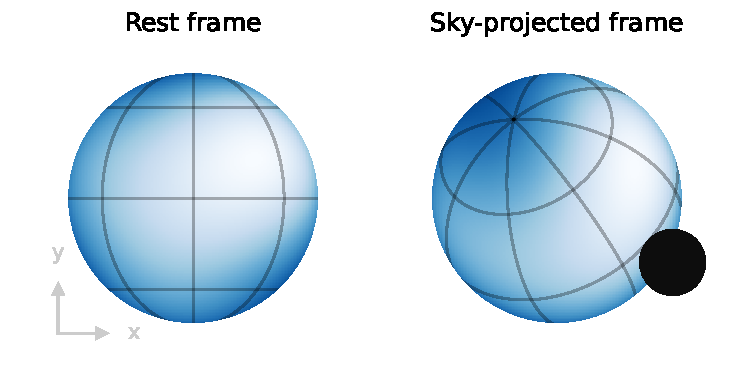
\includegraphics[width=0.6\textwidth]{../workflows/rotations/figures/rotation_basis.pdf}
        \caption{Rotation of the spherical harmonics basis to place the star in the sky-projected frame of the observer.}
        \label{fig:rotation_basis}
    \end{center}
\end{figure}

The rotation of spherical harmonics involves the computation of Wigner-D-matrices, commonly obtained through robust recursion relations in both degree $l$ and order $m$, but leading to costly computations. Hence, knowing how to decompose the full spherical harmonics rotation using pre-computed rotations is essential to achieve optimal performance in the \textit{starry} framework. \autoref{fig:rotation_starry} shows the 6 elementary rotations currently used in the \texttt{starry} implementation.
\begin{figure}[H]
    \begin{center}
        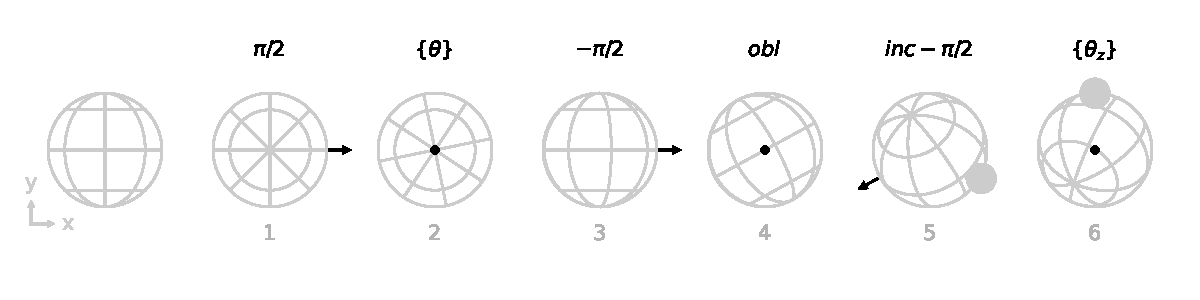
\includegraphics[width=\textwidth]{../workflows/rotations/figures/rotation_starry.pdf}
        \caption{Consecutive rotations of the spherical harmonics basis in the \texttt{starry} implementation. Each schematic shows a sphere rotated from a previous orientation around an axis displayed as a black vector and an angle shown on top.}
        \label{fig:rotation_starry}
    \end{center}
\end{figure}
In this figure, rotations 1 to 3 correspond to a rotation of the star around its rotation axis, and rotations 3 to 5 place the star on a sky-projected frame. Finally, rotation 6 aligns the spherical harmonics map to the occulting body on the $y$ axis in order to apply Green's theorem in the appropriate basis (Figure 2 from \citealt{starry}). The first thing to notice is that rotations 1 to 3 could be simply reduced to a rotation of angle $\theta$ about the y-axis, turning steps 1 to 3 into one. However, rotations around the pole, i.e.\,with a rotation axis along $z$, have simpler expressions that can be implemented separately. In addition, pre-computing these matrices at lower cost is particularly important for steps 2 and 6, involving a potentially large set of angles $\{\theta\}$ and $\{\theta_z\}$, defined over times $\{t\}$, for which to compute the full light curve. This explains the current decomposition of the complete rotation in six separate steps.\\\\
In \texttt{jaxoplanet}, we compute the Wigner-D-matrices by employing the Risbo recursion relations \citep{Risbo1996} implemented in \texttt{JAX} as part of the \texttt{s2fft} Python package \citep{price:s2fft}. In addition, we merge rotations 3, 4 and 5 (see \autoref{fig:rotation_jaxoplanet}) into a single compound rotation of axis
\begin{equation}
    \bvec{v} = \frac{1}{\sqrt{1 - \cos^2{\left(\frac{inc}{2} \right)} \cos^2{\left(\frac{obl}{2}\right)}}} \begin{pmatrix}
        \sin{\left(\frac{inc}{2} \right)} \cos{\left(\frac{obl}{2}\right)}\\
        \sin{\left(\frac{inc}{2} \right)} \sin{\left(\frac{obl}{2}\right)}\\
         - \cos{\left(\frac{inc}{2} \right)} \sin{\left(\frac{obl}{2}\right)}\\
    \end{pmatrix},
\end{equation}
and angle
\begin{equation}
    \omega = 2 \cos^{-1}{\left(\cos{\left(\frac{inc}{2} \right)} \cos{\left(\frac{obl}{2}\right)} \right)}.
\end{equation}
This way, the complete rotation reduces to the four separate steps shown in \autoref{fig:rotation_jaxoplanet}.
\begin{figure}[H]
    \begin{center}
        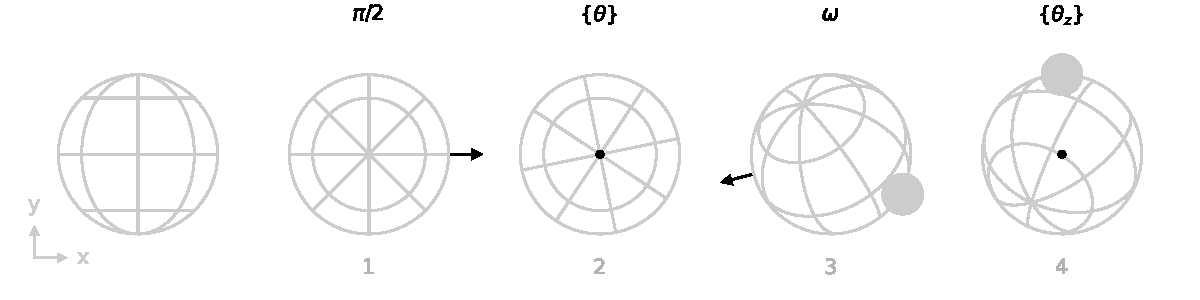
\includegraphics[width=\textwidth]{../workflows/rotations/figures/rotation_jaxoplanet_1.pdf}
        \caption{Consecutive rotations of the spherical harmonics basis in the \texttt{jaxoplanet} implementation. Each schematic shows a sphere rotated from a previous orientation around an axis displayed as a black vector and an angle shown on top.}
        \label{fig:rotation_jaxoplanet}
    \end{center}
\end{figure}

\subsection{Computation of the solution vectors}\label{solution_vectors}

\newpage
\section{Performance}\label{performances}
Although \textit{starry} occultation light curves have analytical expressions, their practical implementation relies on numerical approximations chosen to balance precision and computation time. This is the case, for example, of the solution vector $\bvec{s}$, computed using numerical series expansions in \texttt{starry} (\citealt[section D.2.3]{starry}) and numerical integration in \texttt{jaxoplanet} (see \autoref{solution_vectors}). Other expressions, such as the Wigner-D matrices used in the rotation of the spherical harmonics basis, are computed using reccurence relations prone to the accumulation of numerical errors and instability.\\\\
In this section, we evaluate the accuracy and speed of the \texttt{jaxoplanet} implementation and compare it with the C++ implementation of \texttt{starry}.

\subsection{Precision}
We evaluate the precision of the \texttt{starry} and \texttt{jaxoplanet} terms against quantities computed at arbitrary precision, using a ground truth version of the code implemented with the \texttt{mpmath} Python library\footlink{https://mpmath.org/}. The precision of the overall flux $f$ can only be understood by considering the precision of the terms involved in \autoref{eq:starry}: the solution vector $\bvec{s}$ ($\bvec{r}$ if no occultation), the basis matrices $\bvec{A}$ and $\bvec{B}$, and the Wigner-D rotation tensor $\bvec{R}$. Although we show in \autoref{fig:precision_SAR} that the precision of the \texttt{starry} and \texttt{jaxoplanet} implentations differ for many of these terms, we focus this section on the solution vector $\bvec{s}$ and the overall flux $f$.\\\\
Assuming that we perform the numerical integration of the solution vector $\bvec{s}$ at a relatively high order ($n=500$; see \autoref{solution_vectors}), \autoref{fig:precision_s} shows that our reimplentation of \texttt{starry} reaches relative errors lower than 1 part per billion for $\bvec{s}$ and the overall flux $f$, considering both a small ($r=0.01$) and a large ($r=100$) occultor transiting the star accross numerically-sensitive values of impact parameters $b$. For reference, \autoref{fig:precision_s_starry} shows comparable errors on the same quantities computed with the C++ implentation of \texttt{starry}. In addition, \autoref{fig:precision_degree} shows the evolution of the error on $f$ for increasing degrees of the spherical harmonics, both for \texttt{starry} and \texttt{jaxoplanet}. With these results, we validate the precision of \texttt{jaxoplanet} ans show it is on per with the legacy C++ \texttt{starry} implentation\footnote{version 1.2.0 \citep{starry_120}} described in \cite{starry}.\\\\
\begin{figure}[H]
    \begin{center}
        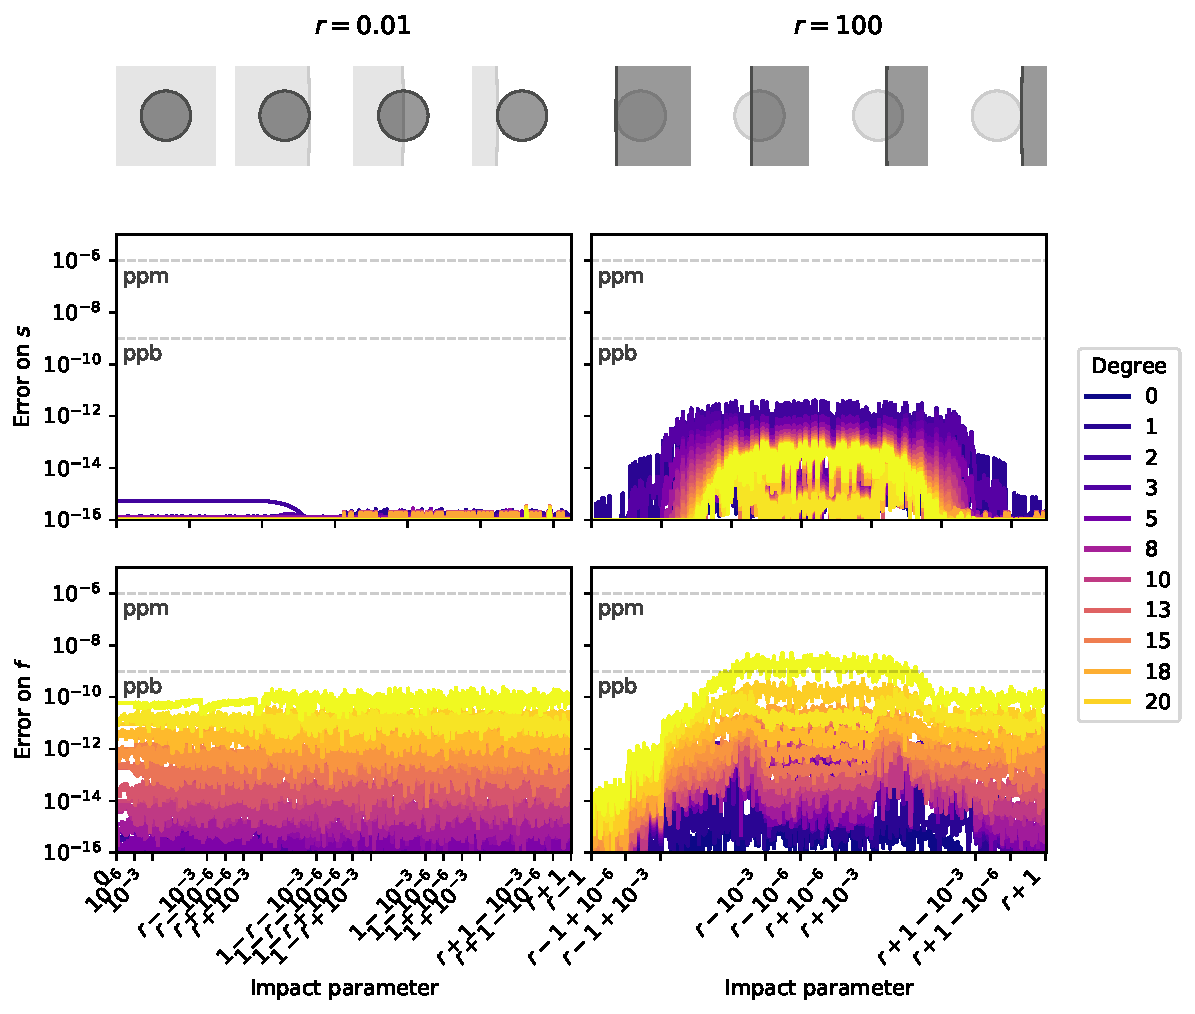
\includegraphics[width=\textwidth]{../workflows/precision/figures/error_jax.pdf}
        \caption{Error of the solution vector $\bvec{s}$ and the overall flux $f$ for all terms of the spherical harmonics basis up to degree $l=20$. Errors are computed against arbitrary-precision computations of $\bvec{s}$ and $f$ for a small ($r=0.01$) and a large ($r=100$) occultor transiting the star accross numerically-sensitive values of impact parameters $b$. For each $(l, m)$ basis component, errors are scaled to the highest values of $\bvec{s}$ (respectively $f$) over $b$. Then, the plotted errors for each degree $l$ are the maximum of the scaled errors over all $m\in [-l, l]$ components over $b$. The disks at the top of the figure show the transit configurations of the occultor (light dark) and the star (light gray) for different values of $b$. \codelink{workflows/precision/scripts/plot_error}}
        \label{fig:precision_s}
    \end{center}
\end{figure}
\begin{figure}[H]
    \begin{center}
        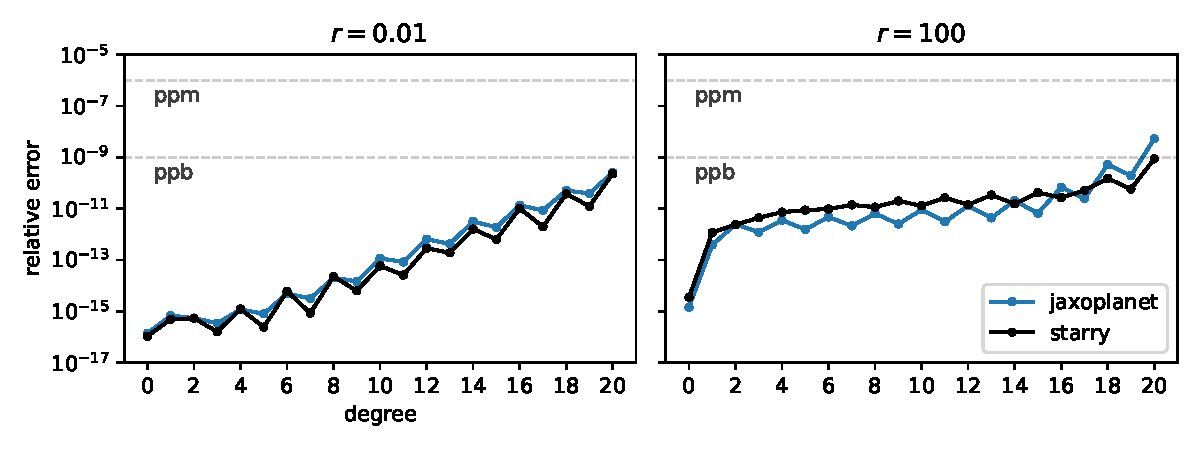
\includegraphics[width=\textwidth]{../workflows/precision/figures/error_degree.pdf}
        \caption{Maximum errors in the overall flux $f$ for all degrees of the spherical harmonics components. Errors shown in this figure correspond to the maximum values of the scaled errors shown in \autoref{fig:precision_s}, maxima taken over the range of values $b$. \codelink{workflows/precision/scripts/plot_error_vs_degree}}
        \label{fig:precision_degree}
    \end{center}
\end{figure}
As described in \autoref{solution_vectors}, we compute \textit{starry} light curves using the Gauss Legendre quadrature to approximate the $\mathcal{P}$ integral involved in the expression of the solution vector $\bvec{s}$. Hence, the precision of the computed flux $f$ depends on the order of the Legendre polynomial which defines the number of points used to approximate $\mathcal{P}$. For this reason, users must carefully set the order parameter to reach the precision required for their application, as shown in \autoref{fig:relative_error_1}.\\\\
\begin{figure}[H]
    \begin{center}
        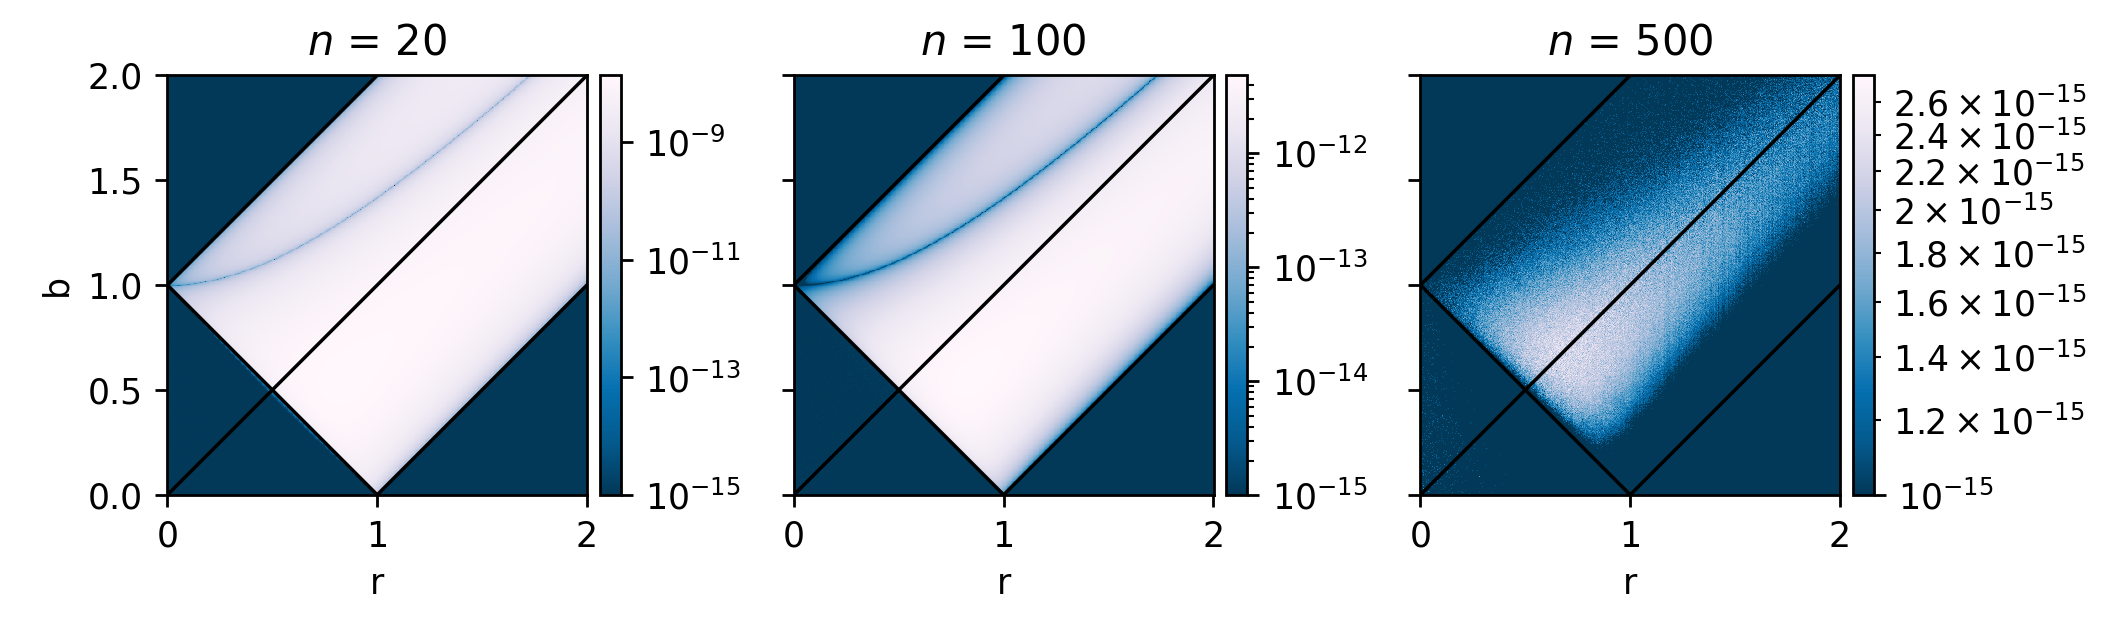
\includegraphics[width=\textwidth]{../workflows/speed/figures/error_rb.png}
        \caption{relative numerical error in the flux $f$ of a linearly limb-darkened star transited by an opaque companion over the $(r, b)$ parameter space. The error is evaluated for different orders $n$ of the Gauss-Legendre quadrature and computed against \texttt{starry} for speed and convenience. Note that \autoref{fig:precision_s} was produced using $n=500$ (right plot) for which $\bvec{s}$ reaches machine precision.}
        \label{fig:relative_error_1}
    \end{center}
\end{figure}
At a fixed occultor radius, \autoref{fig:relative_error_2} shows the time required to compute the flux of the system for a range of $N$ impact parameters $b$, plotted against the maximum relative error reached, the order $n$ of the Gauss-Legendre approximation, and the hardware used for the computation.

% \begin{figure}[H]
%     \begin{center}
%         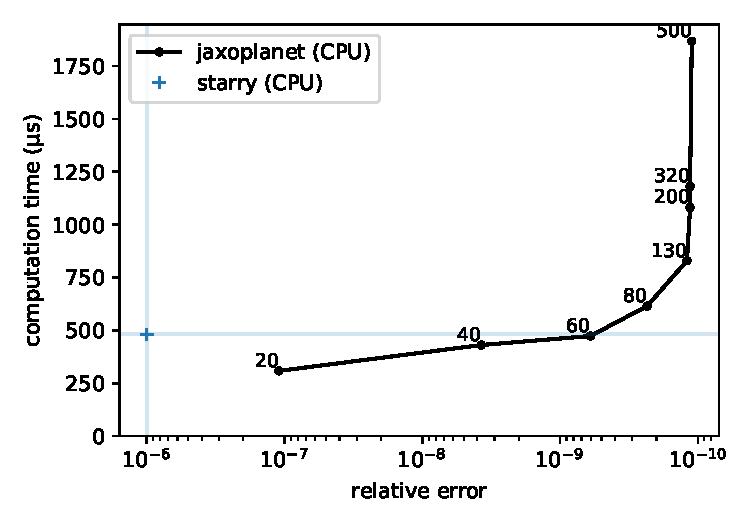
\includegraphics[width=\textwidth]{../workflows/performance/figures/error_vs_time.pdf}
%         \caption{}
%         \label{fig:relative_error_2}
%     \end{center}
% \end{figure}
These computations were run on an apple M1 CPU and an NVIDIA ... GPU. Thanks to the use of JAX, no harware-specific... \\\\



By computing $\mathcal{P}$ numerically, we show that our vectorized implementation reaches machine-precision on a GPU, up to an order of magnitude faster than the current C++ implementation of \texttt{starry} ran on a CPU.\\\\

Plot of the precision versus speed of the computed light curves.

Plot of the solution vectors computation similar to figure 11 and 12 of luger (maybe in the appendix)

\subsection{Speed}\label{speed}



\section{Case study: ...}

\appendix

\section{Error budget}
\begin{figure}[H]
    \begin{center}
        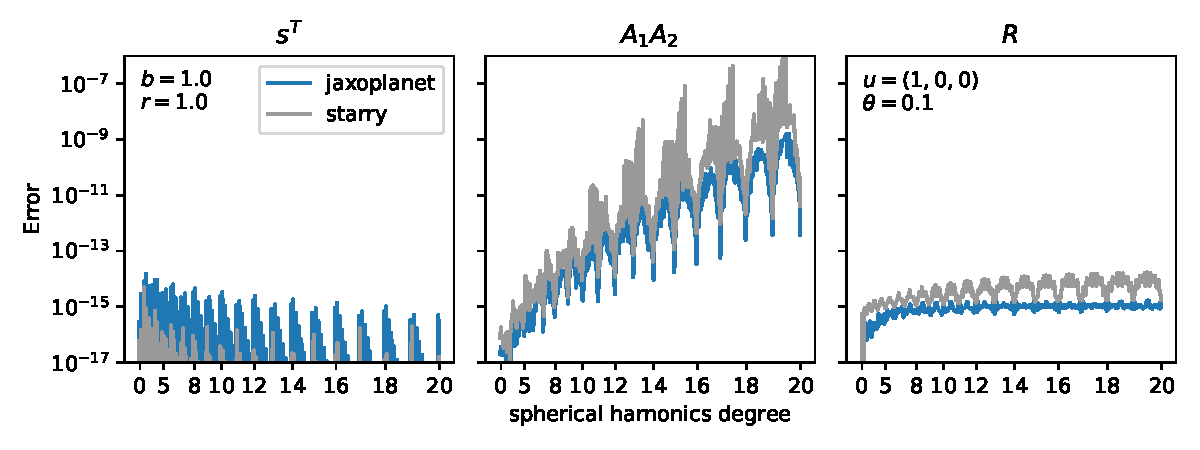
\includegraphics[width=\textwidth]{../workflows/precision/figures/error_SAR.pdf}
        \caption{\codelink{workflows/precision/scripts/plot_error_SAR}}
        \label{fig:precision_SAR}
    \end{center}
\end{figure}

\begin{figure}[H]
    \begin{center}
        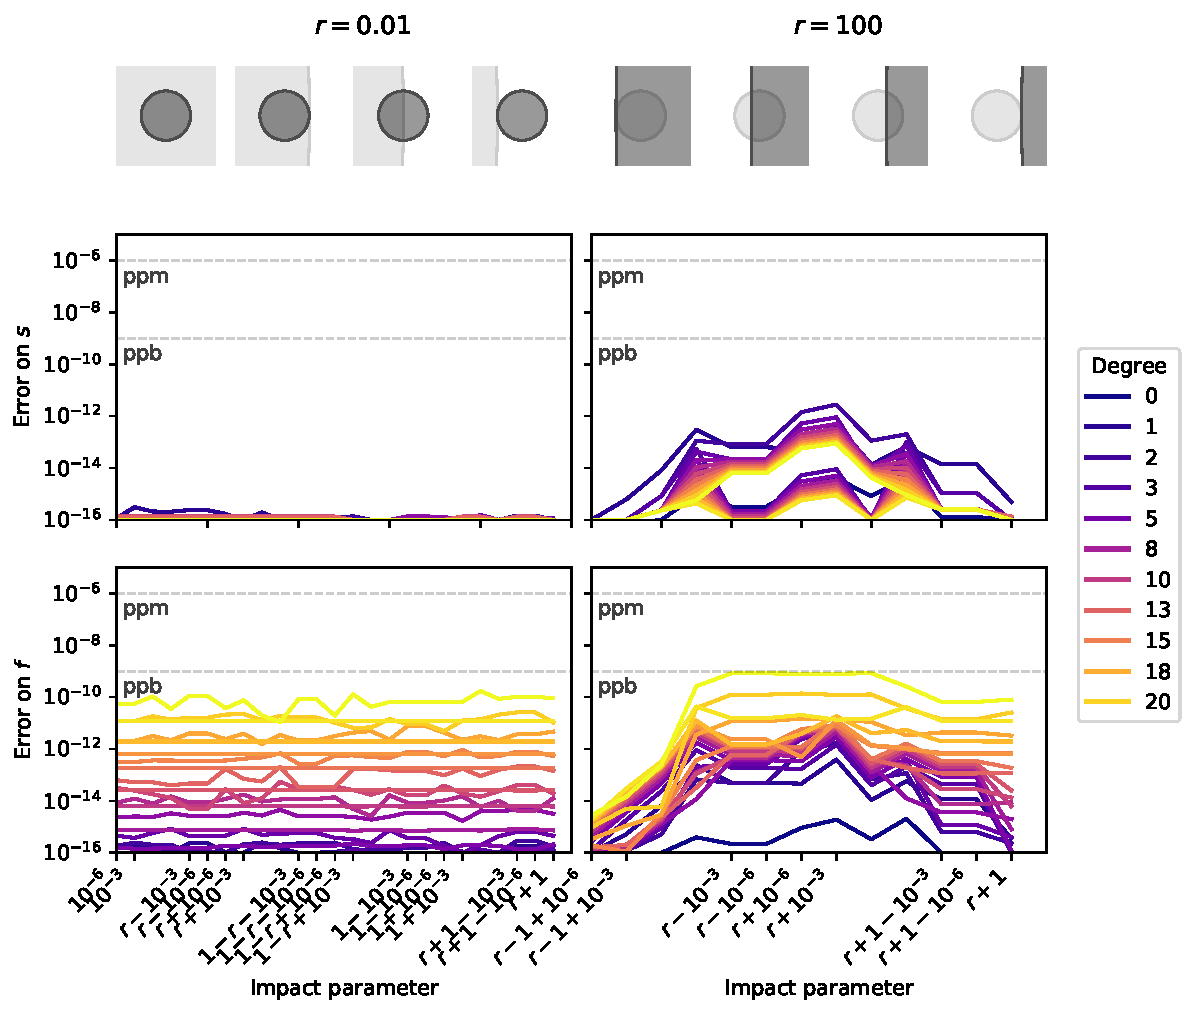
\includegraphics[width=\textwidth]{../workflows/precision/figures/error_starry.pdf}
        \caption{Same as \autoref{fig:precision_s} but with $bvec{s}$ and $f$ computed with the C++ implementation of \texttt{starry}. \codelink{workflows/precision/scripts/plot_error}}
        \label{fig:precision_s_starry}
    \end{center}
\end{figure}

\bibliography{ref}

\end{document}